\documentclass[twoside,twocolumn,9pt,a4paper]{IEEEtran}
\usepackage{graphics,epsfig,amsmath,graphpap}
\usepackage{multirow,cite,hyperref}
%\usepackage[applemac]{inputenc}
\usepackage[utf8]{inputenc}
\usepackage[english]{babel}
\graphicspath{ {./Images/} } % Denna lade jag till som referar så man kan använd folder "Images"
\usepackage{float}
\usepackage{placeins}
\usepackage{placeins}
\usepackage{geometry}

\geometry{top=1.5cm,bottom=1.5cm,left=4cm,right=4cm}

\begin{document}
\onecolumn

\title{Optimum and Adaptive Signal Processing \\
\large Project Description}
\author{Jonathan Olsson (BME21)}
\maketitle
\begin{center}
\line(1,0){350}
\end{center}
\IEEEaftertitletext{\vspace{-1\baselineskip}}

\section{Introduction} \label{secIntroduction}
The data that I've decided to process is BitCoin data from the \href{https://www.nasdaq.com/nasdaq-data-link}{\textit{Nasdaq Data Link}} database.
Nasdaq is a cloud-based technology platform that provides real-time market data and is used by analysts from top-data driven organizations.

\begin{figure}[h]
\begin{center}
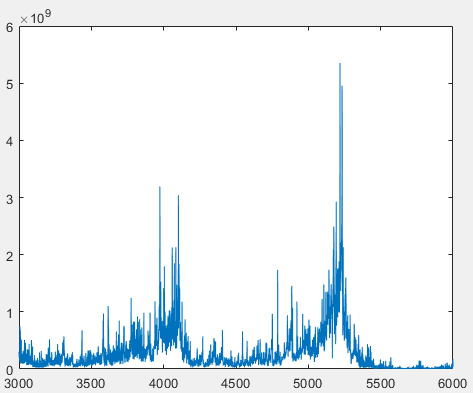
\includegraphics[width=7.5cm]{Images/bitcoin.png} %figurer sparas lämpligen i eps format
\caption{BitCoin prices between 2015-11-02 and 2024-01-19}
\label{DimensionMicrochip}
\end{center}
\end{figure} % Micro chip dimensions 1

The first filter that I'm going to use is an \textit{Adaptive Predictor} that will in theory predict future BitCoin prices. The second filter that I'm going to use is an \textit{Adaptive Moving Average} filter. Due to how volatile BitCoin data is, rapid changes can be
hard to analyze. By using AMA the data can be smoothed while filtering noise.

\end{document}